\documentclass{article}
\usepackage{
    amsmath,
    amssymb,
    mathtools,
    tcolorbox, 
    minted, 
    pgfplots, 
    multirow, 
    graphicx,
    svg
}
\usepackage[a4paper,  total={185mm,260mm}, left=10mm, top=10mm]{geometry}

\usepackage{biblatex} %Imports biblatex package
\addbibresource{refs.bib} %Import the bibliography file

\title{Advanced Digital Systems Design - SVM Acceleration}
\author{Your name (Your Group)} 
\date{March 2024}

\newtcolorbox{obsbox}{
    colback=gray!20, % Grey background color
    colframe=white,  % White frame color (no border)
    title={},        % Empty title
    arc=0pt          % No rounded corners
}

\newtcolorbox{couldbox}{
    colback=purple!20, % Purple background color
    colframe=white,    % White frame color (no border)
    title={},          % Empty title
    arc=0pt            % No rounded corners
}

\usepackage{biblatex} %Imports biblatex package
\addbibresource{refs.bib} %Import the bibliography file

\begin{document}

\maketitle

Some cool ideas from here\cite{expandcordic} and there\cite{vivadoguide}.

% A cool chart comparing values
\begin{figure}[h]
    \centering
    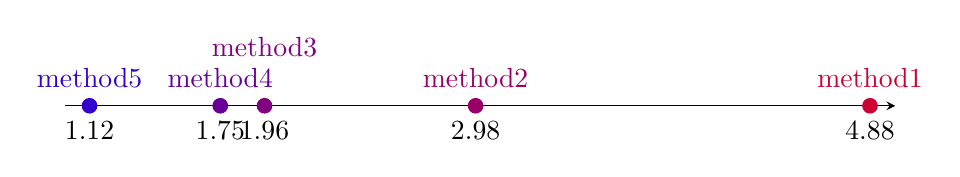
\begin{tikzpicture}
        \begin{axis}[
                xlabel={},
                ylabel={},
                xmin=1, xmax=5,  % Adjust the x-axis range
                ymin=0, ymax=1,  % Adjust the y-axis range
                xtick={1.1183,1.7481,1.9612,2.9782,4.8785},
                width=\textwidth,
                ytick=\empty,
                axis x line=bottom,  % Show x-axis line at the bottom
                axis y line=none,    % Hide y-axis line
                clip=false,
            ]

            % Plot the horizontal line
            \addplot[domain=1:5, dashed, black] {0};  % Horizontal line

            % Place points with text labels    
            \node[label={[above, text=blue!20!red]method1},circle,fill=blue!20!red,inner sep=2pt] at (axis cs:4.8785,0) {};
            \node[label={[above, text=blue!40!red]method2},circle,fill=blue!40!red,inner sep=2pt] at (axis cs:2.9782,0) {};
            \node[label={[above=4mm, text=blue!50!red]method3},circle,fill=blue!50!red,inner sep=2pt] at (axis cs:1.9612,0) {};
            \node[label={[above, text=blue!60!red]method4},circle,fill=blue!60!red,inner sep=2pt] at (axis cs:1.7481,0) {};
            \node[label={[above, text=blue!80!red]method5},circle,fill=blue!80!red,inner sep=2pt] at (axis cs:1.1183,0) {};

        \end{axis}
    \end{tikzpicture}
    \caption{Software time (ms) per image on 2601 image test set}
    \label{fig:softtimes}
\end{figure}


\begin{couldbox}
    \textbf{Potential:} Could have put some cool text here
\end{couldbox}


\begin{obsbox}
    \textbf{Observation:} Some cool things occured \\
    \textbf{Explanation:} I am confidently wrong
\end{obsbox}
\begin{obsbox}
    \textbf{Observation:} Other cool stuff happened.\\
    \textbf{Explanation:} I know, but I lack conviction
\end{obsbox}

\begin{figure}[h]
    \centering
    \begin{tikzpicture}
        \begin{axis}[
                % title={Comparison of Implementations},
                width=\textwidth,
                height=.4\textwidth,
                xlabel={l2Squared},
                ylabel={Output Value},
                ymin=0, % Adjust as needed
                xmin=10, % Adjust as needed
                xmax=10000, % Adjust as needed
                xmode=log,
                legend style={at={(1,1)}, anchor=north east},
                ymajorgrids=true,
                grid style=dashed,
            ]

            \addplot table [mark=none, x=input, y=output, col sep=comma] {data/math.csv};
            \addlegendentry{$exp(-0.001x)$}

            \addplot table [mark=none, x=input, y=output, col sep=comma] {data/flat3354iter3stretch.csv};
            \addlegendentry{$n = 3$, $iters = 7$, zero $>3354.6$}

        \end{axis}
    \end{tikzpicture}
    \caption{Comparison of Implementations of $exp(-0.001x)$ and the modified cordic implementation}
\end{figure}

\begin{obsbox}
    \textbf{Observation:} Squiggly Lines  \\
    \textbf{Explanation:} Maths
\end{obsbox}

Some cool code to distract you
\begin{minted}{cpp}
FIXED_S(15, 8) l2s_sum = 0;
FIXED_U(17, 2) l2Squared = l2s(vert, 0, x);
svs_index_loop: for (int i=1; i<SVS_DIM_2; i++)
    {
        FIXED_U(12, 12) K_root_3 = cordic_exp(l2Squared);
        l2s_sum += alpha3(vert, i-1, K_root_3);
        l2Squared = l2s(vert, i, x);
    }

FIXED_U(12, 12) K_root_3 = cordic_exp(l2Squared);
l2s_sum += alpha3(vert, SVS_DIM_2-1, K_root_3);
return l2s_sum;
\end{minted}

\begin{figure}[h]
    \centering
    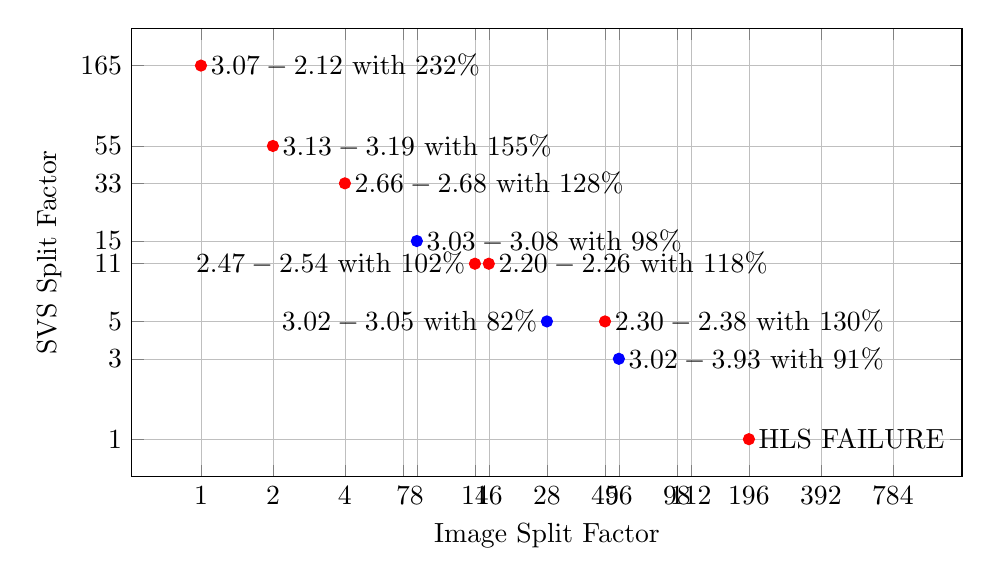
\begin{tikzpicture}
        \begin{axis}[
                xlabel={Image Split Factor},
                ylabel={SVS Split Factor},
                xmode=log,
                ymode=log,
                xmin=0, xmax=784,
                ymin=0, ymax=165,
                width=\textwidth,
                height=.6\textwidth,
                xtick={1, 2, 4, 7, 8, 14, 16, 28, 49, 56, 98, 112, 196, 392, 784},
                ytick={1, 3, 5, 11, 15, 33, 55, 165},
                xticklabels={1, 2, 4, 7, 8, 14, 16, 28, 49, 56, 98, 112, 196, 392, 784}, % Manually specify the xticklabels
                yticklabels={1, 3, 5, 11, 15, 33, 55, 165},
                grid=both,
                grid style={line width=.1pt, draw=gray!10},
                major grid style={line width=.2pt,draw=gray!50},
                only marks, % Show only markers
                mark=*,
                scatter/use mapped color={draw=black, fill=blue}, % Marker color
                % x dir=reverse,
                % y dir=reverse,
                enlargelimits=0.1, % Increase padding
            ]

            \addplot[scatter, mark=*, only marks, scatter src=explicit symbolic, nodes near coords, draw=red, fill=red]  coordinates {
                    (196, 1)
                    (49, 5)
                    (14, 11)
                    (16, 11)
                    (2, 55)
                    (1, 165)
                    (4, 33)
                };
            \addplot[scatter, mark=*, only marks, scatter src=explicit symbolic, nodes near coords, draw=blue, fill=blue]  coordinates {
                    (8, 15)
                    (56, 3)
                    (28, 5)
                };
            \node[anchor=west] at (axis cs:196,1) {HLS FAILURE};
            \node[anchor=west] at (axis cs:56,3) {$3.02-3.93$ with $91\%$};
            \node[anchor=east] at (axis cs:28,5) {$3.02-3.05$ with $82\%$};
            \node[anchor=west] at (axis cs:49,5) {$2.30-2.38$ with $130\%$};
            \node[anchor=east] at (axis cs:14,11) {$2.47-2.54$ with $102\%$};
            \node[anchor=west] at (axis cs:16,11) {$2.20-2.26$ with $118\%$};
            \node[anchor=west] at (axis cs:8,15) {$3.03-3.08$ with $98\%$};
            \node[anchor=west] at (axis cs:2,55) {$3.13-3.19$ with $155\%$};
            \node[anchor=west] at (axis cs:1,165) {$3.07-2.12$ with $232\%$};
            \node[anchor=west] at (axis cs:4,33) {$2.66-2.68$ with $128\%$};

        \end{axis}
    \end{tikzpicture}
    \caption{The Space of potential splittings, each with the total estimated latency (over 2601 images, in millions) with the LUT utilisation}
\end{figure}
\begin{obsbox}
    \textbf{Observation:} Thing get bigger when other thing be smoller \\
    \textbf{Explanation:} Its always just a trade off between having what you want, and having what you need.
\end{obsbox}

\begin{figure}[h]
    \centering
    % Using a drawio diagram as an editable svg
    \includesvg{diagrams/final_design.drawio.svg}
    \caption{The final design diagram showing parallelism.}
\end{figure}

\begin{figure}[h]
    \begin{center}
        \begin{tabular}{l r r r r r}
            \textbf{Name}    & \textbf{BRAM} & \textbf{DSP48E} & \textbf{FF} & \textbf{LUT} & \textbf{URAM} \\
            DSP              & -             & -               & -           & -            & -             \\
            Expression       & -             & -               & 0           & 167          & -             \\
            FIFO             & -             & -               & -           & -            & -             \\
            Instance         & 115           & 150             & 9576        & 29477        & -             \\
            Memory           & 0             & -               & 4480        & 1120         & 0             \\
            Multiplexer      & -             & -               & -           & 13274        & -             \\
            Register         & -             & -               & 189         & -            & -             \\
            \hline
            Total            & 115           & 150             & 14245       & 44038        & 0             \\
            \hline
            Available        & 280           & 220             & 106400      & 53200        & 0             \\
            \hline
            Utilization (\%) & 41            & 68              & 13          & 82           & 0             \\
        \end{tabular}
    \end{center}
    \caption{Resource Utilisation}
\end{figure}

Some other ramblings about fpgas.

\printbibliography

\end{document}